\chapter{Introducción} 
\label{chap:intro}

\vspace{-0.2cm}
\comments{Veo que sólo existe una tabla: igual no tiene sentido dejar
  el índice de tablas.}
\lsection{Motivación del proyecto}

El derecho a la privacidad en Internet es algo que todo usuario
debería valorar y, por desgracia, \modified{el gran público no le da
  la importancia que debería \cite{book:PrivacyBigDataPublicGood}.}
\comments{Las citas forman parte del texto: se deben escribir como una
  parte más de la frase y, por tanto, estarán antes del signo de
  puntuación.}

\comments{Me sigue quedando un poco flojo este inicio de texto. Diría
  algo en esta línea: Tal y como refiere la OECD, la protección y
  defensa de la privacidad son piezas fundamentales para el desarrollo
de la democracia en la (cada vez menos) nueva era digital. Es cada vez
más habitual que deleguemos la custodia de nuestra información en
terceras partes, lo que en determinados casos puede suponer una
violación de nuestros derecho a la privacidad.}

No son pocas las noticias que están apareciendo últimamente sobre
empresas como Google relacionadas con la invasión a la
privacidad. Esto, en gran parte, se ha visto incrementado debido a la
llegada de los \textit{smartphones} al mercado(algo relativamente
reciente, hace alrededor de 10 años). El poder llevar en nuestro
bolsillo todo un ordenador tiene el inconveniente de que grandes
empresas como las anteriormente mencionadas pueden tener acceso a
información en tiempo real de nosotros, como por ejemplo a la hora a
la que nos levantamos, la localización de nuestra propia casa e
incluso la ubicación real en todo momento (y sí, de poco sirve
deshabilitar la ubicación por GPS en tu smartphone~\cite{article:GPSTracking} pues también la
pueden averiguar mediante el inicio de sesión en una red WiFi).
\comments{Te falta alguna referencia, por ejemplo,
  \url{https://techcrunch.com/2017/11/21/android-devices-seen-covertly-sending-location-data-to-google/}. También
es relevante tener en cuenta esto: \url{https://wigle.net/}. Permite
geolocalizar usuarios a través de los SSID. }

Por otro lado está el tema de las redes sociales. Con el auge de
Facebook, Instagram y Twitter, gran parte de la población (en el caso
de Norteamérica, casi dos terceras partes) tiene perfil propio en la
plataforma Facebook \modified{(ver Figura~\ref{fig:FBStats})}.

\begin{figure}[h]
	\centerline{
		\mbox{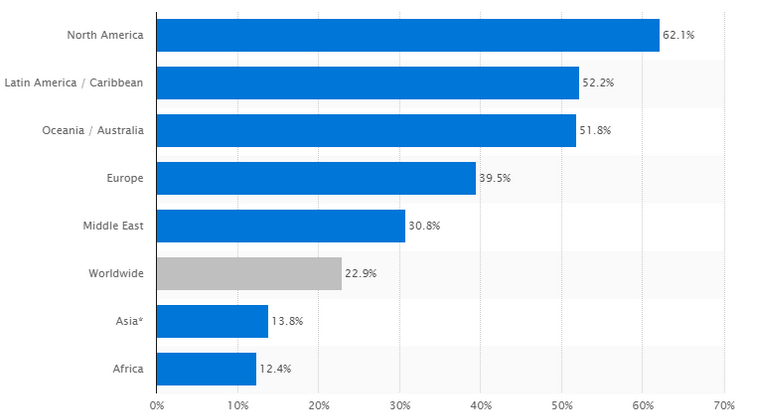
\includegraphics[width=4.00in]{images/sn.png}}
	}
	\caption{Porcentaje de población con perfil en Facebook~\cite{article:FacebookStats} }
	\label{fig:FBStats}
\end{figure}

\comments{Bueno, en realidad el problema viene cuando alguien utiliza
  la información que cedes a un servicio para algo distinto para lo
  que diste permiso. Este tipo de amenaza puede concretarse a través
  de ataques de ingeniería social que permiten agregar información
  desde distintas fuentes (por ejemplo, perfiles de redes sociales) \cite{hadnagy2010social}, o
por comportamientos negligentes o vulneración de los compromisos de
servicio por parte del proveedor. }
Esto de por sí no es un dato negativo, el problema viene cuando para
realizar un registro en una página (como por ejemplo, la web de un
diario), la forma más sencilla es conectando con tu perfil personal de
Facebook. Esto causa que, al interaccionar con dicha página\commented{ (ya sea
publicando un comentario, o cualquier tipo de actividad)} \comments{he
visto que sueles olvidar el espacio antes de los paréntesis. Verifica esto.}, te
arriesgues a que aparezca tu nombre real, con todo lo que ello
conlleva. Desde este punto, saber todo acerca de ese usuario es tan
sencillo como buscar en Google su nombre completo y entrar a su perfil
de Facebook, donde aparecen fotos, su dirección, entre otros (por
suerte, esto es algo que desde hace poco podemos
evitar~\cite{article:GDPRGoogle} gracias a la recientemente adoptada
Ley de Protección de Datos europea, \modified{respecto} a la cual se hará hincapié en este
documento).
\comments{En realidad, la GDPR no evita el problema, sanciona si
  existe tal problema. }

En otros casos el iniciar sesión con la cuenta de Google o Facebook
sirve para que dichas empresas conozcan mejor tus gustos y
\commented{hobbies} \comments{mejor aficiones, o ponerlo en
  cursiva. Los neologismos deben aparecer en cursiva, en caso de que
  no exista traducción. Si existe traducción, es preferible que figure
la misma.},
para así ofrecerte publicidad a medida. \comments{Esta circunstancia
  no tiene por qué suponer una erosión de nuestra privacidad, de forma
que sólo se configura como tal en aquello supuestos en los que el
proveedor de servicios no respeta los términos que el usuario aceptó
para disfrutar el servicio en cuestión \cite{diaz2015privacy}. Es más, no siempre es
necesario llevar a cabo una identificación biunívoca de un usuario
para proporcionar un servicio y garantizar unos niveles de protección
de una plataforma. En efecto, es factible identificar usuarios de
forma anónima y pseudo-anónima \url{https://privacypass.github.io/},
sin que eso imposibilite un debido control de acceso y una necesaria
monitorización de actividad de usuario.}

\comments{Sigue siendo díficil captar tu mensaje. Intentaría ser más
  claro. Algo en esta línea}\modified{De acuerdo con todo lo anterior, parece
  claro que la navegación por el denominado ciberespacio no está
  exenta de peligros. Si en el mundo físico podemos sufrir robos, en
  el ciberespacio igualmente podemos sufrir sustracción de datos y
  suplantación de nuestra identidad. De hecho, una gran parte de los
  problemas que surgen  en el ciberespacio vienen derivados por la
  complejidad asociada a la conversión de nuestra identidad física en
  identidad digital, esto es, la identidad en base a la cual somos
  validados como usuarios legítimos de una cierta aplicación o de un
  cierto servicio. Esta conversión se realiza normalmente por una
  tercer parte o entidad en la que confiamos para gestionar nuestra
  identidad (digital) y proporcionarnos los permisos y privilegios
  necesarios para utilizar una aplicación o servicio. Este marco
  operativo descansa, pues, sobre un modelo de confianza que no
  siempre es satisfecho \ldots}
\comments{Como digo, algo en esta línea, pero con tus propias
  palabras. Además, apóyate en dos cuestiones fundamentales en
  seguridad y privacidad, y que veo que no aparecen reflejadas en la
  actual versión del texto. A saber, el principio de mínimo privilegio 
y \cite{schneider2003least} el consentimiento informado \cite[Capítulo
1]{lane2014privacy}. Es decir, a una entidad (en este caso, proveedor
de servicio) se le dará sólo la información que necesita para realizar
su tarea (i.e., prestarnos  el servicio), para lo cual se dará
consentimiento expreso en el momento que se accede a hacer uso de tal
servicio. En el caso concreto de servicios de almacenamiento en la
nube, por ejemplo, nosotros damos permiso a manejar nuestra identidad
para controlar el acceso a nuestros archivos, y sólo confiamos en el
proveedor de servicios como mecanismos fiable de custodia de la
confidencialidad de nuestros datos \cite{sanchez2018review}. }

La motivación de este proyecto reside tanto en un estudio de diversas
tecnologías para proteger la privacidad de un usuario mediante el
anonimato como en identificar un conjunto de técnicas que suponen una
amenaza para nuestra privacidad.
 
Parte de la motivación también reside mi interés en el ámbito de la
seguridad informática. Es un tema de suma importancia (algo que puede
apreciarse en la creciente demanda de expertos en ciberseguridad hoy
en día~\cite{article:expCiberseguridad}) y además sirve para poner en
práctica metodologías y lenguajes estudiados en el grado.

En definitiva, el proyecto abarca un software modular compuesto de
varias herramientas funcionales por sí mismas y donde además el
requisito principal es la seguridad del
sistema(\textit{security-by-design}~\cite{paper:secbydesign}), y sobre
todo que dicho sistema respete la privacidad del usuario
(\textit{privacy-by-design}~\cite{paper:privacybydesign}
~\cite{cavoukian2009privacy}). Además, este requisito pasará a ser
obligatorio a partir de que entre en vigor \commented{la ya mencionada
  GDPR} \comments{en el texto principal todavía no la has
  mencionada. Añade, por otra parte, referencia al texto de la GDPR.}, por
lo que las empresas desarrolladoras de software deberán tener en
cuenta la privacidad de los datos de cada usuario en las fases de
diseño de todos los proyectos.


\lsection{Objetivos y enfoque}

Principalmente se pretenden lograr dos objetivos fundamentales en este proyecto.

El primero es el de hacernos conocedores más a fondo de las diferentes
vías a la hora de anonimizarnos en Internet, las variadas herramientas
que pretenden conseguir este objetivo (así como las que pretenden
identificar a un usuario), \modified{así como de las diferentes
  nociones} del término
privacidad~\cite{article:danezis2010}. \comments{Te conviene destacar
  algo en esta línea $\rightarrow$ En este último punto, conviene
  destacar que este trabajo está fundamentalmente concernido con la
  dimensión tecnológica de la privacidad. Así, en el presente texto no
  se abordará el debate vigente en el ámbito legal entre las
  consideraciones de la privacidad desde la óptica estadounidense
  (privacidad como secreto, \emph{privacy-as-secrecy}) y la valoración
  de la privacidada en clave europea (privacidad como derecho
  inalieable del sujeto físico, \emph{privacy-as-personhood})
  \cite{solove2002conceptualizing}.} En conclusión, \modified{el
  presente proyecto trata} realizar una investigación exhaustiva sobre
la \modified{dimensión tecnológica} privacidad y los caminos para
asegurarla.

Por otro lado, y quizá el objetivo más importante, es el de poner en
práctica los conocimientos adquiridos en la investigación
anteriormente dicha. En este caso se ha diseñado, desarrollado y
probado una herramienta con numerosas y diversas funciones, cuyo
principal propósito es el de \modified{proporcionarnos una experiencia
  de navegación en Internet} lo más
anónima posible en todo momento.




\lsection{Metodología y plan de trabajo}

Este documento se organiza de la siguiente manera:
\begin{itemize}
	\item Estado  del  Arte: El segundo capítulo explica todos y cada uno de los conceptos de los que trata este proyecto, es decir, el término privacidad, anonimato y la importancia de los mismos hoy en día. Además, se mostrarán ejemplos de herramientas y metodologías para anonimizarse. 
	\item Análisis: El capítulo tres consta de la serie de requisitos, definidos  según  los objetivos  deseados  en  las  aplicaciones  finales  y  delimitados  por  el  alcance  del proyecto.La funcionalidad de la herramienta desarrollada se resume tanto en el catálogo de requisitos como de casos de uso.
	\item Diseño: Este capítulo trata con detalle la fase de diseño, teniendo en cuenta la estructura de la aplicación y el flujo de navegación de la misma 
	\item Desarrollo: En el quinto capítulo se encuentra explicado el método de desarrollo, las librerías utilizadas, los lenguajes en los que está programada la herramienta, las características Software del equipo de desarrollo y el porqué de dicha elección.
	\item Integración, pruebas y resultados: Aquí se tratan las pruebas unitarias realizadas, así como los resultados de las mismas y cómo se han integrado todos los módulos en la aplicación final.
	\item Conclusiones/Trabajo  futuro: Por último, en este capítulo resumimos las conclusiones de la aplicación y el futuro trabajo que se requeriría para que la herramienta continúe creciendo.
\end{itemize}

\newpage \thispagestyle{empty} % Página vacía 